\documentclass[aps,pra,10pt,twocolumn,groupedaddress,nofootinbib]{revtex4-1}

\usepackage{amsmath, amssymb, amsthm}
\usepackage{graphicx}% Include figure files
\usepackage{bm,bbm}% bold math
\usepackage{hyperref}% add hypertext capabilities
\usepackage[margin=2cm]{geometry}
\usepackage{xcolor}
\usepackage{algorithm}
\usepackage[noend]{algpseudocode}
\usepackage{qcircuit}

\theoremstyle{plain}
\newtheorem{theorem}{Theorem}%[section]


\DeclareMathOperator{\re}{Re}
\DeclareMathOperator{\im}{Im}
\DeclareMathOperator{\tr}{Tr}
\DeclareMathOperator{\Ad}{Ad}
\DeclareMathOperator{\ad}{ad}
\DeclareMathOperator{\diag}{diag}  % diagonal vector of the given matrix / diagonal matrix with the given vector as diagonal
\DeclareMathOperator{\Ker}{Ker}    % kernel
\DeclareMathOperator{\Imag}{Imag}  % image
\DeclareMathOperator{\spec}{spec}  % eigenvalue spectrum
\DeclareMathOperator{\lcm}{lcm}    % least common multiple

\newcommand{\isom}{\cong} % isomorphic to
\newcommand{\conj}[1]{\overline{#1}} % complex conjugate
\newcommand{\mnorm}[1]{\ensuremath{\left\| #1 \right\|}} % matrix norm

\newcommand{\de}[2]{\frac{d #1}{d #2}}   % derivative
\newcommand{\pd}[2]{\frac{\partial #1}{\partial #2}}  % partial derivative
\newcommand{\hc}{\text{h.c.}}  % hermitian conjugate

\newcommand{\be}{\begin{equation}}
\newcommand{\ee}{\end{equation}}
\newcommand{\bpm}{\begin{pmatrix}}
\newcommand{\epm}{\end{pmatrix}}

\newcommand{\naturals}{\ensuremath{\mathbb N}}
\newcommand{\Z}{\ensuremath{\mathbb Z}}  % integer numbers
\newcommand{\Q}{\ensuremath{\mathbb Q}}  % rational numbers
\newcommand{\R}{\ensuremath{\mathbb R}}  % real numbers
\newcommand{\C}{\ensuremath{\mathbb C}}  % complex numbers
\newcommand{\K}{\ensuremath{\mathbb K}}  % any field
\newcommand{\I}{\mathbbm{1}} % vector space identity op

\newcommand{\SL}{\text{SL}} % special linear group
\newcommand{\GL}{\text{GL}} % general linear group
\newcommand{\OO}{\text{O}}  % orthogonal group
\newcommand{\SO}{\text{SO}} % special orthogonal group
\newcommand{\U}{\text{U}}   % unitary group
\newcommand{\SU}{\text{SU}} % special unitary group
\newcommand{\Sp}{\text{Sp}} % symplectic group


\newcommand{\CNOT}{\text{CNOT}}

\newcommand{\comm}[2]{\ensuremath{\left[#1, #2\right]}}             % commutator
\newcommand{\acomm}[2]{\ensuremath{\left\{#1, #2\right\}}}          % anticommutator
\newcommand{\ket}[1]{\ensuremath{\left| #1 \right \rangle}}
\newcommand{\bra}[1]{\ensuremath{\left \langle #1 \right |}}
\newcommand{\braket}[2]{\ensuremath{\left\langle #1\left|#2 \right.\right\rangle}}
\newcommand{\ketbra}[2]{\ket{#1}\bra{#2}}
%\newcommand{\vect}[1]{\ensuremath{\mathbf{#1}}}
\newcommand{\inprod}[2]{\ensuremath{\left\langle #1, #2 \right\rangle}}  % inner product
\newcommand{\lieprod}[2]{\ensuremath{\left[#1, #2\right]}}          % Lie product
\newcommand{\liealg}[1]{\ensuremath{\mathfrak{#1}}}                 % Lie algebra
\newcommand{\expect}[1]{\ensuremath{\left\langle #1 \right\rangle}} % expectation value
\newcommand{\tracep}[1]{\ensuremath{\trace\left( #1 \right)}}


\renewcommand{\a}{\hat{a}}
\newcommand{\adag}{\hat{a}^{\dagger}}
\newcommand{\x}{\hat{x}}
\newcommand{\p}{\hat{p}}
\renewcommand{\c}{\hat{c}}
\renewcommand{\d}{\hat{d}}
\newcommand{\bx}{\mathbf{x}}
\newcommand{\bp}{\mathbf{p}}
\newcommand{\bq}{\mathbf{q}}
\newcommand{\e}{\mathrm{e}}
\newcommand{\bad}{\bm{\hat a}^\dagger}
\renewcommand{\L}{\mathcal{L}}
\newcommand{\G}{\mathcal{G}}
\newcommand{\cR}{\mathcal{R}}

\newcommand{\sidenote}[1]{\marginpar{\footnotesize{\textcolor{red}{-#1}}}}

\newcommand{\nathan}[1]{\textcolor{blue}{Nathan: #1}}
\newcommand{\maria}[1]{\textcolor{orange}{Maria: #1}}
\newcommand{\ville}[1]{\textcolor{purple}{Ville: #1}}
\newcommand{\cg}[1]{\textcolor{cyan!80!black}{Christian G.: #1}}

%quantum and classical node stypes
\usepackage{tikz}
\usetikzlibrary{calc}
\usetikzlibrary{shapes.multipart}
\definecolor{quantum1}{HTML}{8EDBCE}
\definecolor{quantum2}{HTML}{3F605B}
\definecolor{exp1}{HTML}{9AB9ED}
\definecolor{exp2}{HTML}{204177}
\definecolor{classical}{HTML}{EBBA92}
\tikzset{input node/.style={}}
\tikzset{quantum node/.style={draw, align=center, anchor=west, inner sep=5pt,rounded corners=4pt, rectangle split, rectangle split horizontal, rectangle split parts=2, rectangle split part fill={quantum1,quantum2}, every two node part/.style={text = white}}}
\tikzset{classical node/.style={draw, rectangle,align=center, anchor=west, thin, fill=classical, inner sep=5pt}}
%\tikzset{expectation node/.style={draw, align=center, anchor=west, inner sep=5pt, rectangle split, rectangle split horizontal, rectangle split parts=2, rectangle split part fill={exp1,exp2}, every two node part/.style={text = white}}}
\tikzset{output node/.style={}}
\tikzset{out label/.style={midway, above}}
\tikzset{connector/.style={anchor=center, opacity=0.}}
\tikzset{samples label/.style={at start, below, xshift=4pt}}


\begin{document}

\title{OpenQML - Technical manuscript}
\author{Maria Schuld}
\author{Nathan Killoran}
\email{nathan@xanadu.ai}
\author{Ville Bergholm}
\affiliation{Xanadu Inc., 372 Richmond St W, Toronto, M5V 1X6, Canada}


\date{\today}

\begin{abstract}
Compilation of formulas and conventions for the OpenQML framework.
\end{abstract}

\maketitle


\section{Model structure}

We consider an abstract \textbf{model} $f(x, \theta)$
that maps a set of \textbf{model inputs} $x$ (which may be empty) and a set of \textbf{model parameters} $\theta$ to a \textbf{model output} $y$. \\

Each set of model parameters $\theta$ is associated with a scalar \textbf{cost} $C(\theta, \mathcal{D})$ of the model, which also depends on a (possibly empty) dataset $\mathcal{D}$.\\

The models we are interested in are hybrid, since they are combinations of quantum and classical computations. Such a model can be depicted as a directed graph of \textbf{nodes} which we call a \textbf{hybrid model graph}. There are two types of nodes: \textbf{Classical nodes} map node inputs $x_c$ and node parameters $\theta_c$ to outputs $y_c$ via a computation executed by a classical computer. \textbf{Quantum nodes} map node inputs $x_q$ and node parameters $\theta_q$ to the estimate of an expectation $y_q$.\\

Each node defines a map from \textbf{node inputs} to \textbf{node outputs}, where the node inputs are the node outputs from the parent nodes. Root nodes (those without parents) take a subset of the model inputs $x$ as node inputs, and the collection of leaf nodes (those without children) return the model output as their node outputs.

\subsection{Quantum nodes}
A quantum node always consists of a \textbf{variational circuit} $U(\gamma)$, where $U$ is a \textbf{quantum circuit} with a set of tunable \textit{circuit parameters} $\gamma$. The circuit acts on an \textbf{initial state} $|\psi_0 \rangle$ which is usually the vacuum state $\ket{0}$.\\

The circuit parameters $\gamma$ can be of three different types: \textbf{trainable parameters} that are associated with the trainable model parameters  $\theta_q$, \textbf{fixed parameters} which are always set to a specific value during training, or \textbf{placeholders} for inputs $x_q$ from preceding classical nodes (if there are any). After applying the variational circuit, we get a final quantum state $\ket{\psi (x_q, \theta_q) }$ from which we draw sample observations with regards to an observable $O$ (i.e., a compuational basis measurement returns samples of bit strings, and a photon number resolution measurement returns strings of integers). The samples are used to estimate the expectation value
\[\gamma \mapsto \bra{\psi_0} U(\gamma)^{\dagger}  \hat{O} U(\gamma) \ket{\psi_0}.\]
The estimation is the output $y_q$ of the quantum node. It is associated with an error
\[ \epsilon = \frac{\langle O \rangle}{\sqrt{R}}, \]
that depends on the variance of the operator $\langle O \rangle$, as well as the number of samples $R$ that we draw. $R$ is a hyperparameter of the quantum node. We draw quantum nodes as:\\
\begin{figure}[h]
\centering
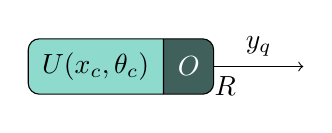
\begin{tikzpicture}
\node[quantum node] (c) at (0,0) {$U(x_c, \theta_c) $ \nodepart{two} $O $};
\draw[->] (c) -- (3.5,0)  node[out label] {$y_{q}$} node[samples label] {$R$};
\end{tikzpicture}
\end{figure}


The variational circuit can be composed of \textbf{layers}
\[ U (\gamma) = \L_{N_L} \cdots \L_{1}\]
which repeat a fixed architecture, which possibly depends on hyperparameters. If there is no layer structure, we set $N_L=1$. A layer $\L_l$, $l=1,...,N_L$, consists of a series of \textbf{gates}
\[\L_l = \G^l_{N_G}(\gamma^l_{N_G}) \cdots \G^l_1(\gamma^l_1). \]
Each gate is parametrised by a set of circuit parameters
$\gamma^i_j$, $i = 1,...,N_L$, $j=1,...,N_G$. The set can be empty if the gate is constant.\\

We propose to use the following \textbf{elementary gate sets} from which the gates $\mathcal{G}$ are taken.

\subsubsection{Qubit architectures}

For qubit architectures we define three parametrized gates,
the elementary rotations around the $x$, $y$ and~$z$ axes:
\begin{eqnarray*}
        R_x(\alpha) &=& \e^{-i\alpha \sigma_x/2} =
        \begin{pmatrix}
          \cos \frac{\alpha}{2} & -i \sin \frac{\alpha}{2}\\
          -i \sin \frac{\alpha}{2} & \cos \frac{\alpha}{2}
        \end{pmatrix}\\
        R_y(\beta) &=& \e^{-i\beta \sigma_y/2} =
        \begin{pmatrix}
          \cos \frac{\beta}{2} & -\sin \frac{\beta}{2}\\
          \sin \frac{\beta}{2} & \cos \frac{\beta}{2}
        \end{pmatrix}\\
        R_z(\gamma) &=& \e^{-i\gamma \sigma_z/2}=
        \begin{pmatrix}
          \e^{-i \frac{\gamma}{2}} & 0\\
          0 & \e^{i \frac{\gamma}{2}}
        \end{pmatrix}\\
\end{eqnarray*}
Any $\SO(3)$ rotation can be expressed using three Euler angles, that is, three rotations around two orthogonal axes. A standard axis choice is~$zyz$. Due to the isomorphism $\SU(2)/\Z_2 \isom \SO(3)$ we obtain a similar \maria{similar to what?} \cg{I suppose similar to how one could/would decompose arbitrary rotations in $\mathbb R^3$ into such around the axes. Maybe mentioning the isomorphism is not even necessary. It is not so hard to see that every element of $SU(2)$ is of the form $
  \begin{pmatrix}
    a & b^*\\
    -b & a^*
  \end{pmatrix}
$ with $|a|^2 + |b|^2 = 1$ and that all such matrices can be reached with the expression below.} decomposition
for arbitrary single-qubit gates $S$:
\begin{align}
\label{eq:app:euler}
\notag
S &= R_z(\gamma) R_y(\beta) R_z(\alpha)\\
&=
\bpm
e^{-i(\alpha+\gamma)/2} \cos(\beta/2) & -e^{i(\alpha-\gamma)/2} \sin(\beta/2)\\
e^{-i(\alpha-\gamma)/2} \sin(\beta/2) &  e^{i(\alpha+\gamma)/2} \cos(\beta/2)
\epm.
\end{align}

Together with the $\CNOT$ gate this gate set is universal, i.e. any $\SU(2^n)$
gate can be expanded into a finite sequence of $\SU(2)$ and $\CNOT$ gates~\cite{barenco1995}.

\subsubsection{CV architectures}

Most gates in CV quantum computing are naturally parametrised. We consider a universal gate set consisting of a universal Gaussian gate set and a nonlinear gate. The following gates are universal for Gaussian transformations,
\begin{eqnarray}
  	R(\phi) & =& \exp\left(i \phi \adag \a \right), \\
  	D(\alpha) & =& \exp(r (e^{i\phi} \adag -e^{-i\phi} \a)), \\
  	S(r) & =& \exp \left(\frac{r}{2} \left(e^{-i\phi} \a^2 -e^{i\phi}  (\adag)^2 \right) \right), \\
  	BS(\theta) & =& \exp\left(\eta (e^{i \phi} \adag_1 \a_2 -e^{-i \phi}\a_1 \adag_2) \right).
  \label{Eq:gaussiangates}
\end{eqnarray}
As the nonlinear gate we consider a general transformation
\begin{equation}
	\mathcal{N}(\phi) = \exp(i \phi \; \varphi(\a, \adag))
	\label{Eq:nonlineargate}
\end{equation}
where $\varphi$ is at least of third order in the quadrature operators.
\cg{A pedantic comment: Not every non-linear gate always promotes linear optics to universality \cite{Oszmaniec2017}.}

\subsection{Classical nodes}

A classical node can be any differentiable function $y_c = h(x_c, \theta_c)$ that maps inputs $x_c$ and model parameters $\theta_c$ to real \maria{any need for complex outputs?} output vectors or scalars $y_c$.\\

We depict classical nodes by the following symbol:\\
\begin{figure}[h]
\centering
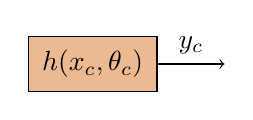
\begin{tikzpicture}
\node[classical node] (c) at (0,0) {$h(x_c, \theta_c) $};
\draw[->] (c) -- (2.5,0)  node[out label] {$y_{c}$};
\end{tikzpicture}
\end{figure}


\begin{figure*}[t]
\begin{flushleft}
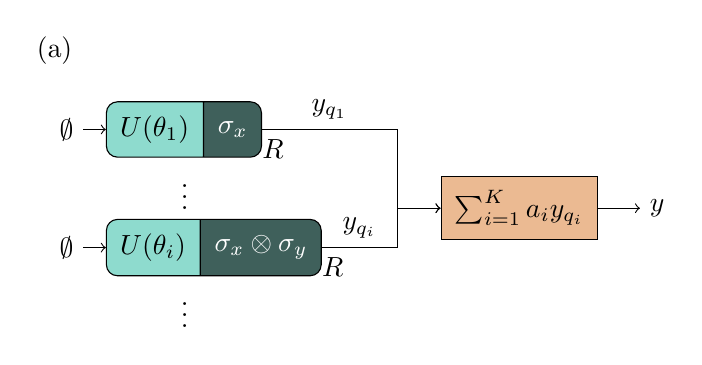
\begin{tikzpicture}
\node[align=left, anchor=west] at (-1,1) {(a)};
\node[input node] (i1) at (-0.5,0) {$\emptyset$};
\node[input node] (iK) at (-0.5,-1.5) {$\emptyset$};
\node[quantum node] (q1) at (0,0) {$U(\theta_1) $ \nodepart{two} $\sigma_x$};
\node[]  at (1,-0.75) {$\vdots $};
\node[quantum node] (qK) at (0,-1.5) {$U(\theta_i)$ \nodepart{two} $\sigma_x \otimes \sigma_y$};
\node[]  at (1,-2.25) {$\vdots $};
\node[classical node] (c) at (4.25,-1) {$\sum_{i=1}^K a_i y_{q_i} $};
\node[output node] (o) at (7,-1) {$y$};
\draw[->] (i1) -- (q1);
\draw[->] (iK) -- (qK) ;
\draw[] (q1.east) -- (3.7,0)  node[out label] {$y_{q_1}$} node[samples label] {$R$};
\draw[->] (3.7,0) -- (3.7,-1)-- (c);
\draw[] (qK.east) -- (3.7,-1.5) node[out label] {$y_{q_i}$} node[samples label] {$R$};
\draw[->] (3.7,-1.5) -- (3.7,-1)-- (c);
\draw[->] (c) -- (o);
%\draw[red] (q1) -| (mid) |- (c.west);
\end{tikzpicture}
 ~~~~~~~~~~~~~~~ 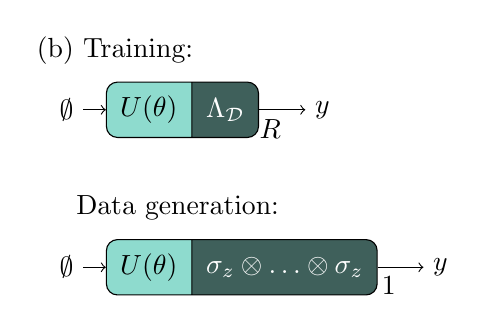
\begin{tikzpicture}
\node[align=left, anchor=west] at (-1,0) {(b) Training:};
\node[input node] (i) at (-0.5,-0.75) {$\emptyset$};
\node[quantum node] (q) at (0,-0.75) {$ U(\theta) $ \nodepart{two} $\Lambda_{\mathcal{D}}$};
\node[output node] (o) at (2.75,-0.75) {$y$};
\draw[->] (i) -- (q);
\draw[->] (q) -- (o) node[samples label] {$R$};
\node[align=left, anchor=west] at (-0.5,-2) {Data generation:};
\node[input node] (i) at (-0.5,-2.75) {$\emptyset$};
\node[quantum node] (q) at (0,-2.75) {$ U(\theta) $ \nodepart{two} $\sigma_z \otimes \hdots \otimes\sigma_z$};
\node[output node] (o) at (4.25,-2.75) {$y$};
\draw[->] (i) -- (q);
\draw[->] (q) -- (o) node[samples label] {$1$};
\end{tikzpicture}\\ \bigbreak

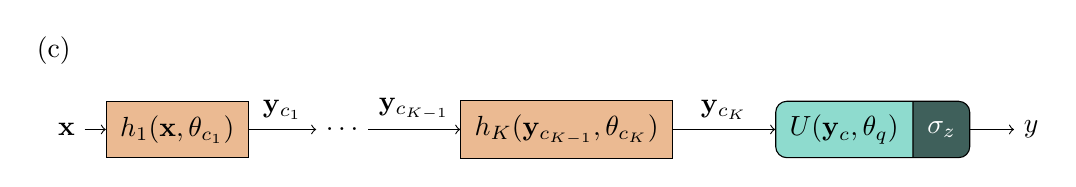
\begin{tikzpicture}
\node[align=left, anchor=west] at (-1,1) {(c)};
\node[input node] (i) at (-0.5,0) {$\bx$};
\node[classical node] (c1) at (0,0) {$h_1(\bx, \theta_{c_1}) $};
\node[] (dots) at (3,0) {$\hdots $};
\node[classical node] (cK) at (4.5,0) {$h_K(\mathbf{y}_{c_{K-1}}, \theta_{c_K}) $};
\node[quantum node] (q) at (8.5,0) {$ U(\mathbf{y}_c, \theta_q) $ \nodepart{two} $\sigma_z$};
\node[output node] (o) at (11.75,0) {$y$};
\draw[->] (i) -- (c1);
\draw[->] (c1) -- (dots) node[out label] {$\mathbf{y}_{c_1}$};
\draw[->] (dots) -- (cK) node[out label] {$\mathbf{y}_{c_{K-1}}$};
\draw[->] (cK) -- (q) node[out label] {$\mathbf{y}_{c_K}$};
\draw[->] (q) -- (o);
\end{tikzpicture}\\ \bigbreak


\end{flushleft}
\caption{Examples of model graphs. Turqois nodes depict quantum nodes, and orange nodes depict classical nodes. (a) Model graph of a variational quantum eigensolver, in which expectation values of local Pauli operators are combined by a classical layer to an expectation value of a global Hamiltonian. (b)  A model, here a generative model) can even have different architectures for training and data generation. While the model is trained maximising the expectation of a quantum operator $\Lambda_{\mathcal{D}}$ that projects onto a `training set subspace' of Hilbert space, it can be used to sample data by performing a single computational basis measurement (i.e., $R=1$). (c) Model graph of a classical neural network with a final quantum layer that computes the scalar output.}
\label{Fig:example_modelgraphs}
\end{figure*}


From the building blocks of classical and quantum nodes, more complicated hybrid structures evolve. Examples of hybrid model graphs are given in Figure \ref{Fig:example_modelgraphs}. Figure \ref{Fig:example_modelgraphs} (a) shows a variational quantum eigensolver, where the model input is an empty set, and the output of the model is the weighed sum of expectation values. Figure \ref{Fig:example_modelgraphs} (b) shows a generative quantum model. Finally, Figure \ref{Fig:example_modelgraphs} (c) shows a classical neural network with one final quantum layer, whose output is the expectation value of a $\sigma_z$ operator applied to a predefined qubit.

\section{Optimization}


\subsection{Cost function}
We consider three different tasks for OpenQML: optimization, unsupervised learning and supervised learning. The tasks depend on whether and what type of data is used for training (see Table \ref{Tbl:tasks}).\\

\begin{table}[t]
\begin{tabular}{lll}
\hline \hline
Task & Inputs & Targets\\
\hline
Optimisation & No & No \\
Unsupervised & Yes & No\\
Supervised & Yes & Yes\\\hline \hline
\end{tabular}
\caption{Definition of the three tasks depending on whether and which type of data is used to train the circuit.}
\label{Tbl:tasks}
\end{table}


The cost function has a different structure for different tasks of training. We will revisit the examples in Figure \ref{Fig:example_modelgraphs} and present some potential cost function for these models. \\

%\begin{figure}[t]
%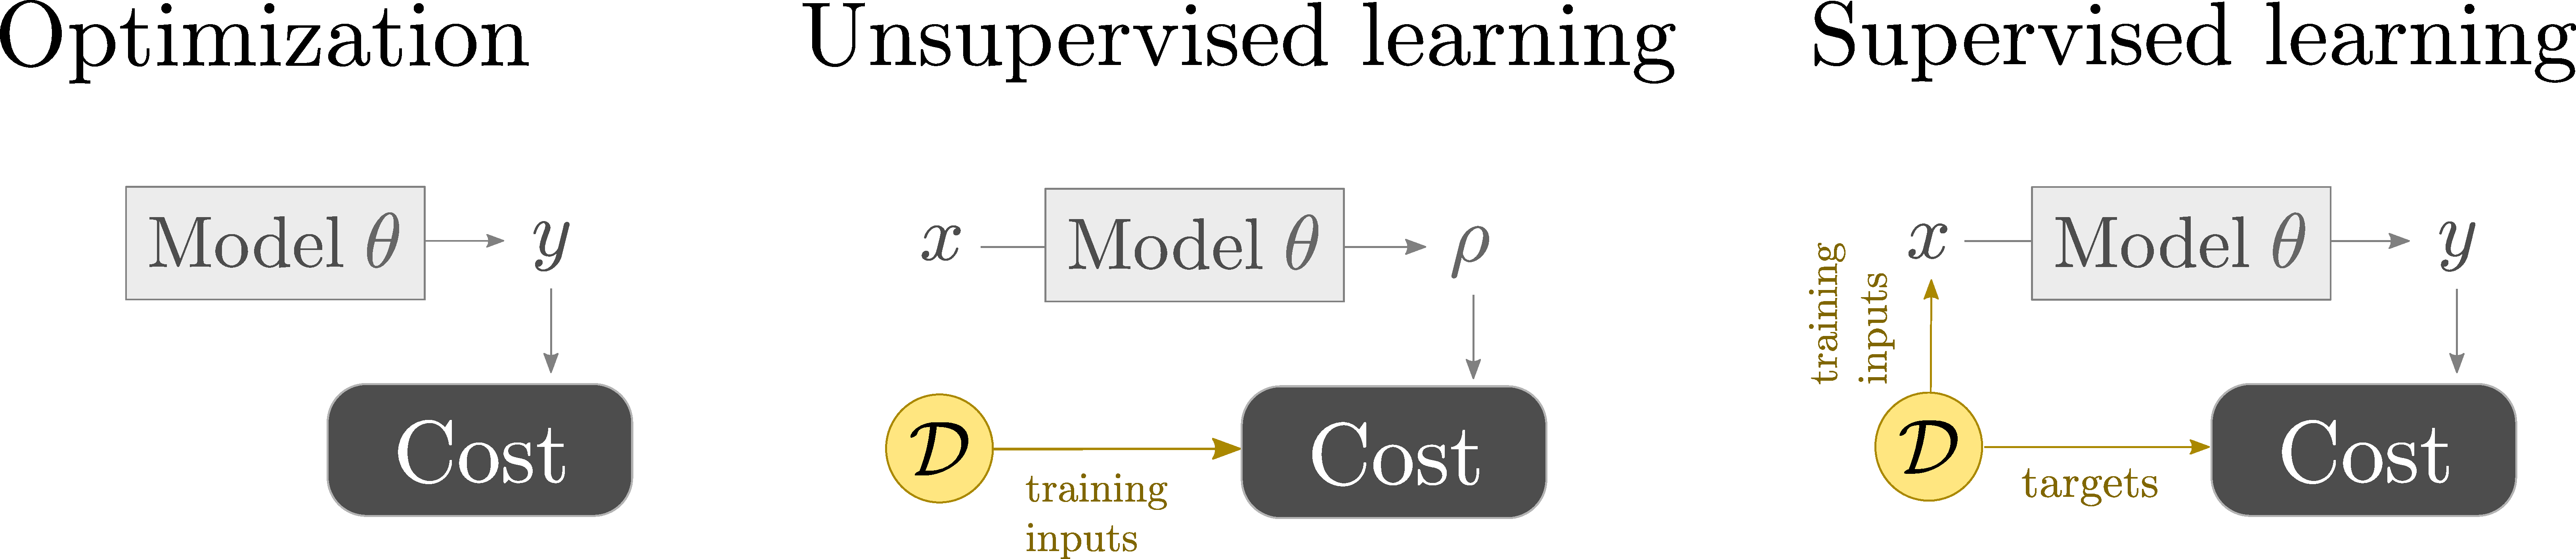
\includegraphics[scale=0.08]{tasks.pdf}
%\caption{Three tasks for OpenQML and the ob}
%\label{Fig:tasks}
%\end{figure}

\paragraph{Expectation maximisation cost for a variational eigensolver}

The cost function of a variational eigensolver is the direct model output $y$ shown in Figure \ref{Fig:example_modelgraphs} (a). $y$ is a weighed sum of local expectation values, which classically computes the expectation value of a global observable which is decomposed into a sum of local observables. Hence, the cost function reads
\[ C(\theta) = \sum_i a_i \bra{0}U(\theta)^{\dagger} O_i U(\theta)\ket{0}, \]
where the $O_i$ are Pauli operators acting on a few qubits only.


\paragraph{Cost for a generative model}
Assume we are given some unlabelled data $\mathcal{D}$ that can be associated with the basis states of a quantum state. Our goal is to prepare a quantum state $\ket{\psi}$ using the variational circuit, so that the likelihood of measuring a basis state $\ket{x^m}$ that represents an input $x^m \in \mathcal{D}$ is large. If we denote the projection onto the basis states that denote the data set as $\Lambda_{\mathcal{D}}$ as in Figure \ref{Fig:example_modelgraphs} (b), the goal is to maximise the expectation of this operator. The loss is hence given by
\[ C(\theta, \mathcal{D}) = \bra{0}U(\theta)^{\dagger} \Lambda_{\mathcal{D}} U(\theta)\ket{0}.\]
\maria{This is not maximum likelihood. Would that be better?}

\paragraph{Square loss cost for supervised learning}
Subfigure (c) in Figure \ref{Fig:example_modelgraphs} is an example of a supervised model. We are given a labelled dataset $\mathcal{D}$. The output $y^m$ of the model for an input $\bx^m$ is defined as the expectation of a specified $\sigma_z$ operator. The square loss compares this expectation with the target value $t^m$ for all training data $m=1,...,M$,
\[ C(\theta, \mathcal{D}) = \sum_{m} |\bra{0}U(\theta, \bx^m)^{\dagger} \sigma_z U(\theta, \bx^m)\ket{0}-t^m|^2. \]

There are of course many other loss functions one could think of, each taking the output of the current model and possibly some data and scoring its parameters with a scalar value.

\subsection{Optimization methods}

There are three methods to optimize models built from classical and quantum nodes:
\begin{enumerate}
\item Gradient-free optimization (i.e., Nelder-Mead, genetic algorithms, particle swarm optimization...)
\item Gradient-based optimization with numerical computation of gradients
\item Gradient-based optimization with analytical computation of the gradients
\end{enumerate}
Note that when we speak of gradients here, we actually refer to estimates of gradients that result from estimates of expectation values. Only in simulations of the quantum circuits can these estimates be exact deterministic values. In the items above, ``analytical computation'' therefore means that if the results of the quantum nodes were exact expectation values (i.e. values derived from analytical computation or estimated by an amount of measurements that goes to infinity), the gradients would be exact. Numerically computed gradients are approximations of the true gradients, even if the quantum nodes were giving exact expectations.

\subsubsection{Gradient-free optimization}
Gradient-free optimization is straight-forward from an algorithmic perspective, since we only need function evaluations that the quantum and classical devices can provide together.

\subsubsection{Gradient-based numeric optimization}

Also numerical methods require only black-box evaluations of the model. The value of the cost function $C(\theta)$ is estimated at two positions close to the current circuit parameter $\mu \in \theta$ which we want to update. The approximation of the gradient is given by
\[ \partial_{\mu} C(\mu) \approx \frac{C(\mu ) - C(\mu + \Delta \mu)}{\Delta \mu} \]
for the \textbf{forward finite-differences} method, and by
\[ \partial_{\mu} C(\mu) \approx \frac{C(\mu - \frac{1}{2}\Delta \mu ) - C(\mu + \frac{1}{2} \Delta \mu)}{\Delta \mu} \]
for the \textbf{centered finite-differences} method. The parameter shift $\Delta \mu$ has to be as small as possible for good approximations, but still large enough to make the finite difference larger than the error in estimating $C(\mu)$ with quantum devices, which makes numerical gradients useless for some applications.

\subsubsection{Gradient-based analytic optimization}

The third method, gradient-based optimization with analytical gradients, takes some more theoretical foundations, which we develop in the following section. The most common algorithm is (stochastic) gradient descent. In gradient descent, to minimize the cost in every \textbf{step} the parameters are updated according to the following simple loop:\\

\begin{algorithmic}[1]
\Procedure{Gradient Descent step}{}
\For {$\mu \in \theta $}
\State $\mu^{(t+1)} = \mu^{(t)} - \eta^{(t)} \partial_{\mu} C(\theta[, \mathcal{D}]) + S$
\EndFor
\EndProcedure
\end{algorithmic}

Here $\mathcal{D}$ is the dataset associated with the cost function for learning problems. If $C$ depends on a dataset $\mathcal{D}$, stochastic gradient descent refers to a gradient descent algorithm where in each step $\mathcal{D}$ is a random subsample of the full training data set. $S$ is an extra term for variations of gradient descent that take momentum (i.e., former gradients) into account. \\

The learning rate $\eta^{(t)}$ can be adapted in each step, either
depending on the gradient or on the step number. $S$ is a potential
additional term that can add a momentum to the update. The gradient
$\partial_{\mu} C(\theta[, \mathcal{D}])$ has to be evaluated by
automatic differentiation of the cost function, which is computed
hybridly by the quantum device or simulator and a classical
computer. We therefore need to define a hybrid automatic
differentiation scheme.




\section{Computing analytical gradients of quantum nodes}

The central feature of OpenQML is that it can compute automatic gradients of expectation values. In this section we therefore explore issues related to computing analytic gradients of models $f(x, \theta)$ consisting of quantum and classical nodes with regards to a specific model parameter $\mu \in \theta$.

\subsection{Gradients of hybrid model graphs}

\subsubsection{Backpropagating throught the graph}

Assume the model $f$ is described by a hybrid model graph $\mathcal{M}$. We want to take the derivative of an element $y_s$ of $f$'s output $y$ with respect to a model parameter $\mu$. Assume that $\mu$ is in the subset $\theta^*$ of the parameters $\theta$, and the subset parametrizes the node $n^*$. For now we assume that the subsets are disjoint, so that there is no parameter tie between nodes. Let $y_s \circ n^{(p)}_1 \circ ... \circ (n^*)^{(p)}$ be the chain of (quantum or classical nodes) that emerges from following the output $y_s$ in the opposite direction of the directed edges until we reach node $n^*$. Since there may be $N_p > 1$ of those paths, we used a superscript to denote the path index. All branches that do not lead back to $\theta_t$ are independent of $\mu$ and can be thought of as constants. We can formally derive a `backpropagation' mechanism for this model.\\

The chain rule prescribes that the gradient with respect to the model parameter $\mu \in \theta_t$ is given by
\[ \partial_{\mu \in \theta_t} y_s = \sum_{p=1}^{N_p} \frac{y}{n_1^{(p)}} \frac{ n^{(p)}_1}{n^{(p)}_{2}}  \cdots \frac{n^*}{\mu}. \]
\cg{I suppose the fractions should be derivatives/gradients?}
\begin{figure}[t]
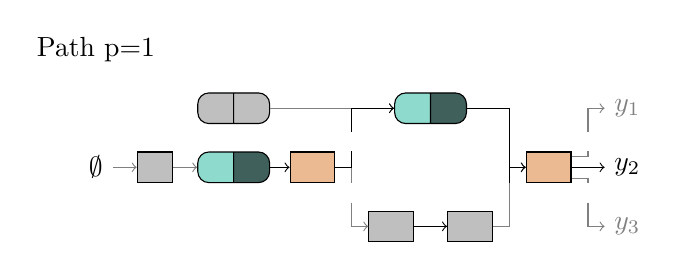
\begin{tikzpicture}
\node[] at (-0.75,1.5) {Path p=1};
\node[input node] (i) at (-0.75,0) {$\emptyset$};
\node[classical node, fill=lightgray, anchor=center] (c1) at (0,0) {\phantom{.}};
\node[quantum node, anchor=center] (q1) at (1,0) {\phantom{.} \nodepart{two} \phantom{.}};
\node[quantum node, fill=lightgray, anchor=center] (q2) at (1,0.75) {\phantom{.} \nodepart{two} \phantom{.}};
\node[classical node, anchor=center] (c2) at (2,0) {\phantom{.} };
\node[anchor=center] (mid1up) at (2.5,0.325) {};
\node[anchor=center] (mid1down) at (2.5,-0.325) {};
\node[quantum node, anchor=center] (q3) at (3.5,0.75) {\phantom{.} \nodepart{two} \phantom{.}};
\node[classical node, fill=lightgray, anchor=center] (c3) at (3,-0.75) {\phantom{.} };
\node[classical node, fill=lightgray, anchor=center] (c4) at (4,-0.75) {\phantom{.} };
\node[anchor=center] (mid2up) at (4.5,0.325) {};
\node[anchor=center] (mid2down) at (4.5,-0.325) {};
\node[classical node, anchor=center] (c5) at (5,0) {\phantom{.} };
\node[anchor=center] (mid3up) at (5.5,0.325) {};
\node[anchor=center] (mid3down) at (5.5,-0.325) {};
\node[output node, anchor=center] (o1) at (6,0.75) {$\textcolor{gray}{y_1}$ };
\node[output node, anchor=center] (o2) at (6,0) {$y_2$ };
\node[output node, anchor=center] (o3) at (6,-0.75) {$\textcolor{gray}{y_3}$ };
\draw[->, gray] (i) -- (c1);
\draw[->, gray] (c1) -- (q1);
\draw[->] (q1) -- (c2);
\draw[->, gray] (q2) -- (q3);
\draw[->, gray] (c2) -| (mid1down)|- (c3);
\draw[->] (c2) -| (mid1up) |- (q3);
\draw[->] (c3) -- (c4);
\draw[->, gray] (c4) -| (mid2up) |- (c5);
\draw[->] (q3) -| (mid2down) |- (c5);
\draw[->, gray] (c5)++(0,4pt) -| (mid3up) |- (o1);
\draw[->] (c5) -- (o2);
\draw[->, gray] (c5)++(0,-4pt) -| (mid3down) |- (o3);
\node[classical node, anchor=center] (c5) at (5,0) {\phantom{.} };

\end{tikzpicture}\\
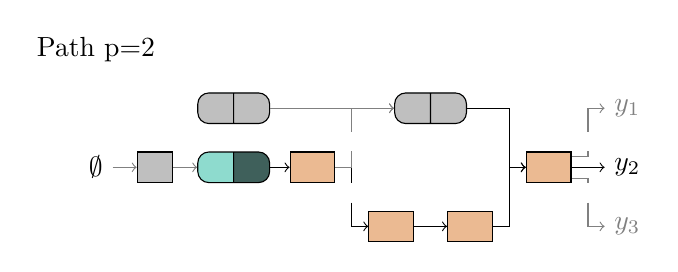
\begin{tikzpicture}
\node[] at (-0.75,1.5) {Path p=2};
\node[input node] (i) at (-0.75,0) {$\emptyset$};
\node[classical node, fill=lightgray, anchor=center] (c1) at (0,0) {\phantom{.}};
\node[quantum node, anchor=center] (q1) at (1,0) {\phantom{.} \nodepart{two} \phantom{.}};
\node[quantum node, fill=lightgray, anchor=center] (q2) at (1,0.75) {\phantom{.} \nodepart{two} \phantom{.}};
\node[classical node, anchor=center] (c2) at (2,0) {\phantom{.} };
\node[anchor=center] (mid1up) at (2.5,0.325) {};
\node[anchor=center] (mid1down) at (2.5,-0.325) {};
\node[quantum node, fill=lightgray, anchor=center] (q3) at (3.5,0.75) {\phantom{.} \nodepart{two} \phantom{.}};
\node[classical node, anchor=center] (c3) at (3,-0.75) {\phantom{.} };
\node[classical node, anchor=center] (c4) at (4,-0.75) {\phantom{.} };
\node[anchor=center] (mid2up) at (4.5,0.325) {};
\node[anchor=center] (mid2down) at (4.5,-0.325) {};
\node[classical node, anchor=center] (c5) at (5,0) {\phantom{.} };
\node[anchor=center] (mid3up) at (5.5,0.325) {};
\node[anchor=center] (mid3down) at (5.5,-0.325) {};
\node[output node, anchor=center] (o1) at (6,0.75) {$\textcolor{gray}{y_1}$ };
\node[output node, anchor=center] (o2) at (6,0) {$y_2$ };
\node[output node, anchor=center] (o3) at (6,-0.75) {$\textcolor{gray}{y_3}$ };
\draw[->, gray] (i) -- (c1);
\draw[->, gray] (c1) -- (q1);
\draw[->] (q1) -- (c2);
\draw[->, gray] (q2) -- (q3);
\draw[->] (c2) -| (mid1down)|- (c3);
\draw[->, gray] (c2) -| (mid1up) |- (q3);
\draw[->] (c3) -- (c4);
\draw[->] (c4) -| (mid2up) |- (c5);
\draw[->] (q3) -| (mid2down) |- (c5);
\draw[->, gray] (c5)++(0,4pt) -| (mid3up) |- (o1);
\draw[->] (c5) -- (o2);
\draw[->, gray] (c5)++(0,-4pt) -| (mid3down) |- (o3);
\node[classical node, anchor=center] (c5) at (5,0) {\phantom{.} };

\end{tikzpicture}
\caption{Illustration of the two paths that lead from the second output $y_2$ back to the first quantum node, with respect to whose parameter we want to differentiate $y_2$.}
\label{}
\end{figure}

This means that we need to be able to compute two types of gradients for each node: The derivative with respect to the input from a previous node, as well as the derivative for each node parameter. Note that while $\partial_{\mu \in \theta_t} y_s$ is a scalar gradient, the gradients in between may be multi-dimensional tensors.\\

The gradients for classical nodes are straight forward, and can be computed by known methods such as (classical) automatic differentiation. However, for quantum nodes this is not obvious. We therefore show how to do quantum automatic differentiation.

\subsubsection{Gradients of quantum nodes}

Quantum nodes map a set of parameters  $\theta_q \subset \theta$ to an estimate of an expectation value $E = \mathrm{tr}\{ \rho(\theta_q ) O\}$ for an operator $O$ with regards to a state $\rho(\theta_q)$ prepared by the variational circuit. For convenience we will drop the subscript $q$ in this section. We will also neglect inputs $x$ to the variational circuit. Derivatives with respect to the node inputs work exactly as if they were model parameters.\\

Formally, we have
\[ \partial_{\mu} \bra{0}U^{\dagger} \hat{O} U \ket{\psi} =  \bra{0}(\partial_{\mu}U^{\dagger}) \hat{O} U \ket{0} + \bra{0}U^{\dagger} \hat{O} (\partial_{\mu} U) \ket{0}, \]

This expression contains the \textbf{circuit derivative},
$\partial_{\mu}  U(\theta)$. Assume that only the $l$th layer depends
on circuit parameter $\mu$, then
\[
\partial_{\mu}  U(\theta) =  \mathcal{L}_1^{\dagger} \cdots (\partial_{\mu} \mathcal{L}_l^{\dagger})\cdots \mathcal{L}_D^{\dagger}.
\]
We call the expression $\partial_{\mu} \mathcal{L}_l^{\dagger}$  the
\textbf{layer derivative}. The layer is decomposed into different
gates from our universal gate set. Let $\mu$ be the parameter of the
$r$th gate $\G_r(\mu)$ (where $\G$ can also depend on other
parameters). The derivative of a layer with respect to $\mu$ is then the product of all the gates, but with $\G_r$ replaced by $\partial_{\mu} \G_r(\mu)$.
This expression
is in general not a quantum gate, and in particular not necessarily a
member of our elementary gate set.

\subsubsection{Gradients of quantum gates}

\maria[FOR NOW MATERIAL IS IN THE APPENDIX]


\section{Error analysis}

Even for analytic differentiation, the gradients are   associated with errors due to the fact that outcomes from quantum nodes are estimates of expectations. This section analyses the propagation and bounds on this error. It also discusses prospects of noise having desirable side effects such as regularisation (known from dropout and similar techniques) and faster convergence of training (as known from Stochastic Gradient Descent training).

\subsection{Error propagation}








%\bibliographystyle{unsrt}
\bibliography{openqml_formalism}

\appendix




\clearpage
\appendix
\section{Gradient computation (Ville)}

In this section we explore issues related to computing gradients of variational quantum circuits.
\ville{Most things in this section are probably not going to make it to the final version,
I'm just organizing my notes on the gradient computation problem here.}


\subsection{Gradient formula for $n$-parameter gates}
\label{sec:gradient_formula_for_n_parameter_gates}
For unitary gates generated by a linear combination of Hermitian generators
$G = \sum_k \theta_k B_k$,
\be
U_{\vec{\theta}} = \exp(-i \sum_k \theta_k B_k) = \exp(-i G),
\ee
we obtain the following formula~\cite{dynamo_manual}:
\be
\pd{}{\theta_k} U_{\vec{\theta}}
= -i \underbrace{\left(B_k +\frac{-i}{2!}\ad_G B_k +\frac{(-i)^2}{3!}\ad_G^2 B_k +\ldots \right)}_{Q_k}
U_{\vec{\theta}}.
\ee
Thus the derivative of the state~$\rho$ propagated by $U_{\vec{\theta}}$ is given by
\begin{align}
  \notag
  \pd{}{\theta_k} \Ad_{U_{\vec{\theta}}} \rho
  &= \pd{}{\theta_k} (U_{\vec{\theta}} \rho U_{\vec{\theta}}^\dagger)
  = \left(\pd{}{\theta_k} U_{\vec{\theta}}\right) \rho U_{\vec{\theta}}^\dagger +\text{h.c.}\\
  %&= -i Q_k U_{\vec{\theta}} \rho U_{\vec{\theta}}^\dagger +\text{h.c.}
  &= -i \ad_{Q_k} \Ad_{U_{\vec{\theta}}} \rho,
\end{align}
where $\Ad_{A} B = A B A^\dagger$ and $\ad_{A} B = A B - B A$.
Assume now we have a propagator U, and the initial state of the system is~$\rho$.
The expectation value of the observable $Q$ is obtained as
\be
\expect{Q}_U = \tr((\Ad_{U}\rho) Q)
= \tr(\rho \Ad_{U^\dagger}Q).
\ee
With $U=B U_{\vec{\theta}} A$, the derivative of the expectation value is given by
\begin{align}
  \label{eq:d_ev}
  \notag
  \pd{}{\theta_k} \expect{Q}_{B U_{\vec{\theta}} A}
  &= \tr(Q \Ad_B (\pd{}{\theta_k} \Ad_{U_{\vec{\theta}}}) \Ad_A \rho)\\
  &= \tr(Q \Ad_B (-i \ad_{Q_k}) \Ad_{U_{\vec{\theta}} A} \rho).
\end{align}

\ville{The usefulness of this formula depends on whether we can sum the series~$Q_k$ easily enough.
  However, evaluating the $\ad_{Q_k}$ part on a quantum computer is the real problem.
}

\subsubsection{One-parameter gates}

In the case where we only have a single generator (one-parameter subgroup, see below),
$G = \theta_1 B_1$, the commutator $\ad_G B_1 = 0$
and the series terminates at the first term, yielding
$Q_1 = B_1$.

\subsubsection{Displacement}

The displacement gate is given by
\begin{align}
  D(\vec{\theta}) &= D(\re z, \im z) = \exp\left( za^\dagger -z^* a\right)\\
  \notag
&= \exp\left(-i\left(\re(z)(-i)(a-a^\dagger) -\im(z)(a+a^\dagger)\right)\right).
\end{align}
The generators are $\{B_k\}_k = \{-i(a-a^\dagger), -(a+a^\dagger)\}$.
Now we have
\begin{align*}
  -i \ad_G B_1 &= -i\comm{i(za^\dagger -z^* a)}{-i(a-a^\dagger)}
  = -2 \theta_2 \I,\\
  -i\ad_G B_2 &= -i\comm{i(za^\dagger -z^* a)}{-(a+a^\dagger)}
  = 2 \theta_1 \I,
\end{align*}
and thus
\begin{align*}
Q_1 &= B_1 -\theta_{2} \I,\\
Q_2 &= B_2 +\theta_{1} \I.
\end{align*}
The series terminate already at the second term, and furthermore
the identity terms do not matter in a commutator.
We obtain $\ad_{Q_k} = \ad_{B_k}$, and
hence displacement gates can be handled exactly the same way as one-parameter gates.
\cg{I guess, another way of seeing this is that different displacements commute. Once can thus always decompose any displacement gate into two commuting one parameter gates, e.g., $D(\re z, \im z) \propto D(\re z, 0) D(0, \im z)$.}

\subsection{One-parameter subgroups in quantum mechanics}

A one-parameter subgroup of the topological group~$G$ is defined by a continuous group homomorphism
\be
\phi: \R \to G,
\ee
where $\R$ is a group with respect to addition.
The homomorphism property means that
\be
\phi(a)\phi(b) = \phi(a+b) \quad \forall a,b \in \R,
\ee
which immediately yields
$\phi(0) = e$ and $\phi(-a) = \phi(a)^{-1}$,
where $e$~is the identity element of~$G$.
$\Imag \phi$ is always a subgroup of~$G$.

The kernel of the homomorphism is defined as
\be
\Ker \phi = \{a \in \R | \phi(a) = e\}.
\ee

\begin{theorem}
  \label{th:1psg}
One-parameter subgroups are either isomorphic to~$\R$, or their parametrization~$\phi$ is periodic.

\begin{proof}
$\phi$ is an injection iff $\Ker \phi = \{0\}$ (trivial kernel).
In this case the subgroup $\phi(\R) < G$ is isomorphic to~$\R$.
Let us next assume that the kernel is nontrivial, i.e. for some $p \neq 0$ we have
$\phi(p) = e$.
% p \in \Ker \phi \implies n*p \in \Ker \phi
This is equivalent to
\be
\phi(a+p) = \phi(a)\phi(p) = \phi(a) \quad \forall a \in \R,
\ee
and the map~$\phi$ is thus periodic. Let us use $\tilde{p}>0$
to denote the period, i.e.
$\tilde{p} = \min \{|p| \neq 0 | p \in \Ker \phi\}$.
Now the kernel is seen to be $\Ker \phi = \{n \tilde{p} | n \in Z\}$.
\end{proof}
\end{theorem}

% https://en.wikipedia.org/wiki/Stone%27s_theorem_on_one-parameter_unitary_groups
Stone's theorem on one-parameter unitary groups states that
% for every strongly continuous one-parameter family of unitary operators on a Hilbert space there is a unique Hermitian generator, and that
for every Hermitian generator~$G$, the homomorphism
\be
\label{eq:1pug}
\phi(\theta) = U_\theta = \exp(-i \theta G)
\ee
defines a strongly continuous one-parameter unitary group.
This holds in both finite-dimensional and infinite-dimensional cases.
The unitary and its generator commute.

\ville{The reason why I'm looking into the periodicity of the subgroup $U_\theta$ is that I was originally
  overoptimistic and though that periodicity might be sufficient to make the gradient trick~\ref{sec:gradient_trick} work. It probably isn't.
  Might be necessary though.}
\cg{Without having thought about it much, I don't expect the periodicity to be relevant for the gradient trick. The intuition is that whether a subgroup is non-periodic or just has a very long period depends on very fine tuned properties of the $\lambda_i$ and so it only matters at long times, whereas the gradient is about infinitesimal changes (This is not a rigorous argument of course). Due to the quantum version of the Poincar\'{e} recurrence theorem, actually, for any $\epsilon$ and any finite dimensional $G$ there is a time $T$ (possibly very large) such that $\|\exp(-i T G) - \I \|_\infty \leq \epsilon$.}

\subsubsection{Finite-dimensional Hilbert spaces}


Assume we are given a hermitian $n \times n$ generator~$G$, with the eigendecomposition
\be
G = V \diag(\lambda_1, \ldots, \lambda_n) V^\dagger.
\ee
%Tracelessness yields $\sum_k \lambda_k = 0$.
%$G$~generates a one-parameter subgroup of the unitary group~$SU(n)$
Now using Eq.~\eqref{eq:1pug} we obtain
\be
U_\theta
= V \diag(e^{-i\lambda_1 \theta}, \ldots, e^{-i\lambda_n \theta}) V^\dagger,
\ee
where $\theta \in \R$. Using Th.~\ref{th:1psg} we find that
\begin{align}
  & U_\theta \: \text{is periodic with period} \: \tilde{\theta} > 0\\
  \iff \: & \Ker U = \{n \tilde{\theta} | n \in Z\}\\
  \iff \: & \lambda_k \tilde{\theta} = n_k 2 \pi \quad \forall k, \: \text{where} \: n_k \in \Z\\
  \iff \: & \frac{\lambda_i}{\lambda_j} = \frac{n_i}{n_j} \quad \forall i,j
  \: \text{for all nonzero eigenvalues.}
\end{align}

Let us extend the definition of least common multiple to real numbers:
\be
\lcm(a_1, a_2, \ldots) := \min \{q | \forall i \exists n_i \in \Z: a_i n_i = q>0\}.
\ee
Such a number exists iff $a_i$ are rational multiples of each other.
Now
\be
\tilde{\theta} = 2\pi \: \lcm \{\lambda^{-1} \:|\: \lambda \in \spec(G) \setminus \{0\}\}.
\ee

In quantum mechanics the global phase of a propagator has no physical meaning, so we may always add
a multiple of identity to the generator~$G$ without affecting the physics.
This is equivalent to shifting all the eigenvalues by the same amount.
Hence the periodicity conditions are relaxed a bit. In particular, we may always make one eigenvalue zero.


Qubits:
$G$~has only two eigenvalues, so $U(\theta)$ is always periodic (modulo the phase)
with $\tilde{\theta} = 2\pi/|\lambda_2-\lambda_1|$.

Qudits:
Now almost all generators~$G$ have eigenvalues that are not rational multiples of each other.
These~$G$ generate a one-parameter subgroup of $U(d)$ isomorphic to~$\R$.
However, some generators~$G$ always generate a periodic subgroup.


\subsection{Attempts at extending the gradient trick}

Let us assume $G$ is such that there is a value~$\theta$ which yields
\be
\label{eq:U_IG}
U_\theta = a\I +bG.
\ee
Adjusting global phase, we may always choose $a \in \R$.
\begin{align}
\label{eq:AdUtheta}
\notag
\Ad_{U_\theta} \rho &=
|a|^2 \rho +\re(ab^*)\acomm{G}{\rho}
-i\im(ab^*)\comm{G}{\rho} +|b|^2 G\rho G\\
&=
a^2 \rho +a\re(b)\acomm{G}{\rho}
+ia\im(b)\comm{G}{\rho} +|b|^2 G\rho G.
\end{align}
\ville{The idea is to add a few of these expressions together with different values of $\theta$
such that only the $\comm{G}{\rho} = \ad_G \rho$ term remains.}

Unitarity also requires
\begin{align}
\notag
&U_\theta U_\theta^\dagger = a^2\I +2\re(ab^*) G +|b|^2 G^2 = \I\\
\iff \:&
2a\re(b) G +|b|^2 G^2 = (1-a^2)\I,
\end{align}
which limits the form $G$ can take.

Another possible approach:
Quite generally we have
\begin{align}
\notag
\Ad_{U_\theta}
&= \Ad_{\exp(-i \theta G)}
= \exp(-i \theta \ad_{G})\\
&= \I +(-i\theta)\ad_G +\frac{(-i\theta)^2}{2!} \ad_G^2 +\ldots
\end{align}
We may eliminate all even terms in the series by projecting to the odd part:
\begin{align}
\notag
\frac{1}{2}\left(\Ad_{U_\theta} -\Ad_{U_{-\theta}})\right)
&= (-i\theta)\ad_G +\frac{(-i\theta)^3}{3!} \ad_G^3 +\ldots
\end{align}


\ville{Can we express $\ad_G$ (for some relevant $G$) using a linear combination of these series expressions with different values of~$\theta$?}

\ville{In the case where $G$ only has two unique eigenvalues, the above series collapses to $\ad_G$ times a scalar sine series, see below.}

\subsection{Gradient trick}
\label{sec:gradient_trick}

Let us assume that $G'$ has only two unique eigenvalues, $\lambda$ and~$\lambda+2r$.
We may now define $G = G' -(\lambda+r)\I$ with the unique eigenvalues
$\pm r$, and obtain $G^2 = r^2\I$.\footnote{
Alternatively we may define $G = G' -\lambda \I$ with the unique eigenvalues
$\{0, 2r\}$, and obtain $G^2 = 2r G$ (a scaled projector).
This yields the same result modulo global phase.}


Now we may write the Taylor series for the exponential
and split it into a cosine and a sine series:
\begin{align*}
U_\theta &= \exp(-iG\theta) = \sum_{k=0}^\infty \frac{(-i\theta)^k G^k}{k!}\\
&=
\sum_{k=0}^\infty \frac{(-i\theta)^{2k} G^{2k}}{(2k)!}
+\sum_{k=0}^\infty \frac{(-i\theta)^{2k+1} G^{2k+1}}{(2k+1)!}\\
&=
\I \sum_{k=0}^\infty \frac{(-1)^{k} (\theta r)^{2k}}{(2k)!}
-i G/r \sum_{k=0}^\infty \frac{(-1)^{k} (\theta r)^{2k+1}}{(2k+1)!}\\
&=
\I \cos(r \theta)
-i G/r \sin(r \theta).
\end{align*}

%For such a scaled idempotent generator we obtain
%\begin{align*}
%U_\theta
%&= \exp(-iG\theta) = \sum_{k=0}^\infty \frac{(-i\theta)^k G^k}{k!}\\
%&= \I +\sum_{k=1}^\infty \frac{(-i\theta)^k (2r)^{k-1}}{k!} G\\
%&= \I +\frac{1}{2r} \sum_{k=1}^\infty \frac{(-i 2r \theta)^k}{k!} G\\
%&= \I +\frac{G}{2r} (\exp(-i 2r \theta)-1).
%\end{align*}


This propagator is of the form presented in Eq.~\eqref{eq:U_IG},
with $a=\cos(r\theta)$ and $b=-i/r \sin(r\theta)$.
All the unwanted terms in Eq.~\eqref{eq:AdUtheta} are seen to be even functions of~$\theta$,
and thus we obtain
\be
\Ad_{U_\theta} -\Ad_{U_{-\theta}}
=
-i r^{-1} \sin(2r\theta) \ad_G.
\ee
The norm of this expression is maximized when $\theta = \pi/(4r)$,
and using the unitary
\be
W := U_{\pi/(4r)} = \frac{1}{\sqrt{2}}(\I -ir^{-1}G)
\ee
we finally obtain the convenient formula
\be
-i\ad_G = r(\Ad_W-\Ad_{W^\dagger})
\ee
which we may use in Eq.~\eqref{eq:d_ev} to compute the gradient of the expectation value.

Qubits:
This trick works for arbitrary single-qubit gates, generated by a linear combination of Pauli matrices
$G = \vec{a} \cdot \vec{\sigma}/2$
where $|\vec{a}|=1$.
We obtain $G^2 = \frac{1}{4} \I$, and thus $r=1/2$.

Qudits (including the multi-qubit case) and CV modes:
Gates generated by a $G$ that has only two unique eigenvalues are amenable to the gradient trick.



\section{Gradient computation (Christian)}
\cg{Hi! I left some comments also in other parts of this manuscript and hope that is ok. Nathan told me to have a closer look at the gradient problem. I don't have any ground breaking insights (and probably you have thought about some of the things I will write below already), but maybe some of the following observations can be useful:}

\ref{sec:gradient_formula_for_n_parameter_gates}

The gradient trick, as described in \ref{sec:gradient_trick}, works for arbitrary generators that are both Hermitian and unitary (or at least unitary up to a constant factor).
In finite dimensional Hilbert spaces, such operators thus have only two different eigenvalues.
Up to rescaling and addition of identities they can thus be transformed into projectors.
Adding identities to generators doesn't change the expectation value and gradient at all (as the global phase does not matter) and rescaling simply rescales the gradient.
The gradient trick, as explained in Section~\ref{sec:gradient_trick}, can thus be straightforwardly applied to all circuits whose gates are generated by projectors (I am not really saying anything new, just paraphrasing what is already explained in the end of Section~\ref{sec:gradient_trick}).

At least for simgle-parameter gates with $G = \theta_1 B_1$ arbitrary hermitian, one can ``extend'' the gradient trick with the following reasoning (spoiler: this is not very practical):
Any hermitian operator $B_1$ can obviously be decomposed in into its eigendecomposition $B_1 = \sum_j b_1^{(j)} \, B_1^{(j)}$ with $b_1^{(j)}$ real and $B_1^{(j)} = {B_1^{(j)}}^2$ commuting orthogonal a projectors and therefore we can write $U_{\theta_1} = \exp(-i \theta_1 \sum_j b_1^{(j)} \, B_1^{(j)}) = \prod_j \exp(-i \theta_1 b_1^{(j)} \, B_1^{(j)}) = \prod_j U^{(j)}_{\theta_1}$.
One can then try to estimate the gradient $\pd{}{\theta_1} \expect{Q}_{B U_{\theta_1} A}$ by ``pretending that that one has actually more parameters'' from estimates of all the $\pd{}{\theta_1^{(j)}} \expect{Q}_{B \prod_k U^{(k)}_{\theta_1^{(k)}} A}$.
In fact, as $2 B_1^{(j)} - \I$ has the right properties to make the gradient trick work, if one can actually perform all the unitaries
\begin{equation}
  W^{(j)} = \frac{1}{\sqrt{2}}(\I - i (2 B_1^{(j)} - \I)) ,
\end{equation}
one can estimate all of these gradients because the general formula \eqref{eq:d_ev} and that fact that all the $B_1^{(j)}$ and $U^{(j)}$ commute imply that
\begin{align}
    \label{eq:d_ev_eigendecomposed}
  &\pd{}{\theta_1^{(j)}} \expect{Q}_{B \prod_k U^{(k)}_{\theta_1^{(k)}}  A} \\
  = &\tr(Q \Ad_{B \prod_{k<j} U^{(k)}_{\theta_1^{(k)}}} ((-i b_1^{(j)}/2) \ad_{2 B_1^{(j)} - \I}) \times\\ &\Ad_{U_{\theta_1^{(k)}} \prod_{k>j} U^{(k)}_{\theta_1^{(k)}} A} \rho)\\
  = &\tr(Q \Ad_B ((-i b_1^{(j)}/2) \ad_{2 B_1^{(j)} - \I}) \Ad_{\prod_{k} U^{(k)}_{\theta_1^{(k)}} A} \rho).     \label{eq:d_ev_eigendecomposed_end}
\end{align}
The linearity of $\ad_{\sum_k b_1^{(k)} B_1^{(k)}} = \sum_k b_1^{(k)} \ad_{B_1^{(k)}}$ and the fact that $\prod_{k} U^{(k)}_{\theta_1^{(k)}} \big|_{\theta_1^{(k)} = \theta_1} = U_{\theta_1}$ then implies that the gradient $\pd{}{\theta_1} \expect{Q}_{B U_{\theta_1} A}$ one is actually interested in, can be recovered as a linear combinations of the gradients in \eqref{eq:d_ev_eigendecomposed} -- \eqref{eq:d_ev_eigendecomposed_end}.
\cg{Well, as I said, this is not very practical.}

\section{Gradient computation (Maria)}
\maria{Adding my attempts and notes here. We can merge the two when ready.}

\subsection{Estimating gradients of expectation values with the LCU technique}

Assume we want to take the derivative of the expectation values
\[ y = \bra{0}U^{\dagger} \G^{\dagger}  V^{\dagger} \hat{O} V \G U \ket{0}\]
of a quantum gate $\G = \G(\mu)$ acting on a single subsystem (i.e., mode or qubit), with respect to the parameter $\mu$ of $\G$. Note that $\G$ could depend on other parameters as well. Here, $U,V$ are the circuits applied before and after this gate. To simplify the notation, we absorb $U$ into the quantum state, and $V$ into the operator and compute $ \bra{\psi} \G^{\dagger}  \hat{Q} \G \ket{\psi}$ instead, with $\hat{Q} = V^{\dagger} \hat{O} V$, and $\ket{\psi}= U \ket{0}$.\\

The derivative of the expectation is formally given by
\begin{equation}
	\partial_{\mu} y = \bra{\psi} ( \partial_{\mu}\G^{\dagger})  \hat{Q} \G \ket{\psi} + \bra{\psi} \G^{\dagger}  \hat{Q}  (\partial_{\mu}\G) \ket{\psi}
	\label{Eq:der_of_exp}
\end{equation}

In matrix notation, the expression $\partial_{\mu}\G$ is the entry-wise gradient of $\G$. Since this is in general a complex square matrix, we can always decompose it into the weighted sum of two unitary matrices $A$ and $B$ [ADD PROOF],
\[\partial_{\mu}\G = \alpha A + \beta B \]
with real $\alpha, \beta$. To be more general, for example if there is a convenient decomposition into more or less than $2$ unitaries, let us assume that
\[\partial_{\mu}\G = \sum_{k=1}^K \alpha_k A_k, \]
for real $\alpha_k$. The gradient becomes
\begin{equation*}
	\partial_{\mu} y  = \sum_{k=1}^K \alpha_k  \left( \bra{\psi} A_k^{\dagger}  \hat{Q} \G \ket{\psi} +  \bra{\psi}\G^{\dagger} \hat{Q} A_k  \ket{\psi} \right).
\end{equation*}
Let us look at one of these terms,
\begin{equation}
	\bra{\psi} A^{\dagger}  \hat{Q} \G \ket{\psi} +  \bra{\psi}\G^{\dagger} \hat{Q} A  \ket{\psi},
\label{Eq:term_to_estimate}
\end{equation}
where here and in the following we drop the subscript $k$ for readability. To estimate this value on a quantum computer, we can instead estimate the two expectations
\begin{equation}
	E_1 = \bra{\psi} (\G + A)^{\dagger} \hat{Q} (\G + A) \ket{\psi},		\label{Eq:E1}
\end{equation}
and
\begin{equation}
	E_2= \bra{\psi}(\G - A)^{\dagger}  \hat{Q} (\G - A) \ket{\psi}
	\label{Eq:E2}
\end{equation}
on the quantum device, and then classically compute $\frac{1}{2}E_1 - \frac{1}{2} E_2$.
\begin{proof}
We have
\begin{eqnarray*}
	E_1 &= &\bra{\psi} \G^{\dagger} \hat{c} \G \ket{\psi} + \bra{\psi} A^{\dagger} \hat{c} A \ket{\psi} \\
	&+& \bra{\psi} \G^{\dagger} \hat{c} A \ket{\psi}+ \bra{\psi} A^{\dagger} \hat{c} \G \ket{\psi}
\end{eqnarray*}
and
\begin{eqnarray*}
	E_2 &= & \bra{\psi} \G^{\dagger} \hat{c} \G \ket{\psi} + \bra{\psi} A^{\dagger} \hat{c} A \ket{\psi} \\
	&-& \bra{\psi} \G^{\dagger} \hat{c} A \ket{\psi}- \bra{\psi} A^{\dagger} \hat{c} \G \ket{\psi}
\end{eqnarray*}
Subtracting the terms cancels the first two expectation values in $E_1$ and $E_2$ and adds the second ones, and the normalisation of $\frac{1}{2}$ ensures that we have the correct normalization.
\end{proof}

We will now propose a way to estimate $E_1$ and $E_2$ using a technique called a linear combination of unitaries (LCU) [REF], first considering a qubit-based quantum computer, and subsequently looking at a CV quantum computer.


\subsubsection{Qubit-based quantum computer}

We will first consider the special case of Pauli rotations, in which the procedure is known to simplify considerably [REF MITARAI], and subsequently consider the more general case.\\

\paragraph{Pauli gates}
Consider the gate $\G(\mu) = \e^{i \mu G}$, where $G$ is hermitian as well as unitary, and therefore a projector, $G^2 = \mathbbm{1}$ [\maria{Tried the more general $G^2 = r \mathbbm{1}$, but ran into trouble with $r$ in the calculation below. Possibly generalise.}]. A prominent example are Pauli operators, and it is known that any single qubit quantum gate can be decomposed into such gates. The gradient of such a gate is given by
\[ \partial_{\mu} \G = i G \e^{i \mu G}.    \]
Then Eq. (\ref{Eq:der_of_exp}) becomes
\[ \partial_{\mu} y =   \bra{\psi} \G^{\dagger} (iG)^{\dagger}  \hat{Q} \mathbbm{1} \G \ket{\psi} + \bra{\psi} \G^{\dagger} \mathbbm{1}  \hat{Q} (iG) \G \ket{\psi} , \]
which has the form of term (\ref{Eq:term_to_estimate}). We can hence write
\[ \partial_{\mu} y = \frac{1}{2}E_1 - \frac{1}{2} E_2, \]
with
\[E_1 = \bra{\psi} (\mathbbm{1} + iG)^{\dagger} \hat{c} (\mathbbm{1} + iG) \ket{\psi},\]
and
\[E_2= \bra{\psi}(\mathbbm{1} - iG)^{\dagger}  \hat{c} (\mathbbm{1} - iG) \ket{\psi}. \]
Since $G$ is a projector, we get
\begin{equation}
	\G(\pm \frac{\pi}{2}) = \frac{1}{\sqrt{2}}(\I \pm iG),
	\label{Eq:Pauli_equality}
\end{equation}

\begin{proof}
We may write the Taylor series for the exponential of $\G(\mu)$
and split it into a cosine and a sine series:
\begin{align*}
\mathcal{G}(\mu) &= \exp(-i\mu G) = \sum_{k=0}^\infty \frac{(-i\mu)^k G^k}{k!}\\
&=
\sum_{k=0}^\infty \frac{(-i\mu)^{2k} G^{2k}}{(2k)!}
+\sum_{k=0}^\infty \frac{(-i\mu)^{2k+1} G^{2k+1}}{(2k+1)!}\\
&=
\I \sum_{k=0}^\infty \frac{(-1)^{k} \mu^{2k}}{(2k)!}
-i G \sum_{k=0}^\infty \frac{(-1)^{k} \mu^{2k+1}}{(2k+1)!}\\
&=
\I \cos(\mu)
-i G \sin(\mu).
\end{align*}
For $\mu = \pm \frac{\pi}{2}$ we get $\G(\pm \frac{\pi}{2}) = \frac{1}{\sqrt{2}}(\I \pm iG)$.
\end{proof}

We conclude that the expectations can be estimated straight from the quantum device, by inserting either a $\G(\frac{\pi}{2})$ or $\G(-\frac{\pi}{2})$ into the original circuit:
\begin{multline*}
	\partial_{\mu} y =   \bra{\psi} \G\left(\mu \right)^{\dagger} \G \left(\frac{\pi}{2} \right)^{\dagger}  \hat{Q} \G\left(\mu \right) \left(\frac{\pi}{2} \right) \G\left(\mu \right) \ket{\psi} \\ + \bra{\psi} \G\left(\mu \right)^{\dagger} \G \left(- \frac{\pi}{2} \right)^{\dagger} \hat{Q} \G \left(-\frac{\pi}{2} \right) \G\left(\mu \right) \ket{\psi}
\end{multline*}

\paragraph{General case}

\begin{figure}[t]
$$
\Qcircuit @C=1em @R=.7em {
\lstick{\ket{0}} &  \gate{H}  &\ctrlo{1} & \ctrl{1}&  \gate{H} & \meter & \cw & \rstick{c}\\
\lstick{\ket{\psi}} &   \qw &\gate{\G} & \gate{A} & \qw  & \qw & \qw & \rstick{\ket{\psi'}}  \\
}
$$
\caption{LCU for qubits.}
\label{Fig:lcu_qubits}
\end{figure}

In the general case we need a trick to estimate expectations (\ref{Eq:E1}) and (\ref{Eq:E2}). One possibility is a linear combination of unitaries [REF].

Prepare the state
\[ \frac{1}{\sqrt{2}} \left( \ket{0} + \ket{1}  \right)\otimes \ket{\psi}, \]
where the first qubit is an ancilla. Now apply $\G$ from Equation (\ref{Eq:term_to_estimate}) conditioned on the ancilla being in state $0$, and $A$ conditioned on the ancilla being in state $1$,
\[ \frac{1}{\sqrt{2}} \left( \ket{0} \G \ket{\psi} + \ket{1} A \ket{\psi} \right). \]
A second Hadamard prepares
\[ \frac{1}{2} \left( \ket{0} (\G + A) \ket{\psi} + \ket{1} (\G - A) \ket{\psi} \right). \]
\maria{This looks nice, but does not help us if I am correct:  $\langle \hat{Q} \rangle = \frac{1}{4} \left( E_1 + E_2 \right) $}
A measurement of the ancilla selects one of the two branches and results in state
$\frac{1}{2 \sqrt{p_0}} (\G + A) \ket{\psi}$ with probability
\[p_0  = \bra{\psi} (\G + A)^{\dagger} (\G + A) \ket{\psi},\]
or in state $\frac{1}{2\sqrt{p_1}} (\G - A) \ket{\psi}$ with probability
\[p_1 = \bra{\psi} (\G - A)^{\dagger} (\G - A) \ket{\psi}.   \]
Note that this is not a conditional measurement: Either result contributes to the final estimate. We measure the expectation of $\hat{Q}$ with respect to the final state. If the ancilla was in state $0$, we contribute the result to the estimation of
\[\tilde{E}_0 =  \frac{1}{4 p_0} \bra{\psi} (\G + A)^{\dagger} \hat{Q} (\G + A) \ket{\psi}, \]
and if the ancilla was in state $0$ we contribute the result towards the estimation of
\[\tilde{E}_1 =  \frac{1}{4 p_1} \bra{\psi} (\G - A)^{\dagger} \hat{Q} (\G - A) \ket{\psi}. \]
We can now use our knowledge of $p_0, p_1$ from the measurement together with $E_0 = 4 p_0 \tilde{E}_0$ and $E_1 = 4 p_1 \tilde{E}_1$ to compute the desired estimate (\ref{Eq:term_to_estimate}), and proceed similarly for the term involving unitary $B$.\\

Overall, on top of the ``normal operation mode'' of the device, this routine requires that we can apply the gate as well the unitaries from the derivative decomposition controlled by an ancilla. We need to estimate $K$ expectation values altogether. Furthermore, the decomposition of the derivative gate into (single-subsystem)  unitaries that can be implemented by the device has to be worked out once. We will show below that for interesting cases in qubit and CV architectures, the $A_k$ are represented by a single qubit gate.


\subsubsection{CV quantum computer}

We show now how to estimate the expectations $E_1, E_2$ for single mode gates on a CV quantum computer. Here, the observables $\hat{O}$ that we are interested in are typically the quadratures $\x, \p$ or the number operator $\hat{a}^{\dagger}\hat{a}$ for a given mode. The LCU circuit is implemented with the help of an additional vacuum mode and beam splitters. We use the Heisenberg picture and will look at the evolution and measurement of the quadratures as an example. As explained above, we consider the observables $\c_1 = V^{\dagger} \x_1 V$ and $\d_1 = V^{\dagger} \p_1 V$, which result from evolving the original quadratures by the circuit $V$ that follows after the gate $\G$. \maria{How can we generalise?} \\

Starting with $\ket{\psi}$ in the first mode (which just means that we already applied circuit $U$), and vacuum in the second, we apply the circuit shown in Fig. \ref{Fig:der_eval_cv}. The circuit consists of a 50-50 beam splitter, a Gaussian transformation on each mode separately, as well as another 50-50 beam splitter. We measure the expectation of the vector of the transformed quadrature operators $\c_1, \d$. \\


\begin{figure}[t]
$$
\Qcircuit @C=1em @R=.7em {
\lstick{\ket{\psi}} &  \multigate{1}{BS(\frac{\pi}{4})}  & \gate{A}&  \multigate{1}{BS(\frac{\pi}{4})} &  \qw \\
\lstick{\ket{0}} &   \ghost{BS(\frac{\pi}{4})}   & \gate{\G}&\ghost{BS(\frac{\pi}{4})} & \qw \\
}
$$
\caption{Derivative evaluation circuit.}
\label{Fig:der_eval_cv}
\end{figure}

The overall quadrature vector is given by
\[\begin{pmatrix} \c_1 \\ \d_1 \\ \x_2 \\ \p_2 \end{pmatrix}, \]
where we use $\x$ and $\p_2$ to describe the quadratures of the second mode (which does not get transformed by a subsequent circuit $V$).
The first beam splitter tranforms this vector to
\[\frac{1}{\sqrt{2}}\begin{pmatrix} \c_1 - \x_2 \\ \d_1 - \p_2 \\ \c_1 + \x_2 \\ \d_1 + \p_2 \end{pmatrix}.\]
The Gaussian gates applied to each mode can be expressed by symplectic transformations applied to the subspaces of each mode. Let the symplectic trafo describing gate $A_k$ acting on the first mode be given by
\[\underbrace{\begin{pmatrix} s_{11} & s_{12}\\ s_{21} & s_{22} \end{pmatrix}}_{S} \begin{pmatrix} \c_1 - \x_2 \\ \d_1 - \p_2 \end{pmatrix} + \underbrace{\begin{pmatrix} \alpha_1 \\ \alpha_2 \end{pmatrix}}_{\alpha}, \]
and let the trafo describing gate $\G$ acting on the second mode be given by
\[\underbrace{\begin{pmatrix} r_{11} & r_{12}\\ r_{21} & r_{22} \end{pmatrix}}_{R} \begin{pmatrix} \c_1 + \x_2 \\ \d_1 + \p_2 \end{pmatrix} + \underbrace{\begin{pmatrix} \beta_1 \\ \beta_2 \end{pmatrix}}_{\beta}.\]
Overall, the evolution is given by
\[\frac{1}{\sqrt{2}}\begin{pmatrix} S & 0 \\ 0 & R \end{pmatrix}
\begin{pmatrix} \c_1 - \x_2 \\ \d_1 - \p_2 \\ \c_1 + \x_2 \\ \d_1 + \p_2 \end{pmatrix} + \begin{pmatrix}\alpha_1\\ \alpha_2 \\ \beta_1 \\ \beta_2 \end{pmatrix}.\]
This yields
\[\frac{1}{\sqrt{2}}\begin{pmatrix} s_{11}(\c_1 - \x_2) + s_{12}(\d_1 - \p_2) + \alpha_1 \\ s_{21}(\c_1 - \x_2) + s_{22}(\d_1 - \p_2)  + \alpha_2 \\ r_{11}(\c_1 + \x_2) + r_{12}(\d_1 + \p_2)  + \beta_1 \\ r_{21}(\c_1 + \x_2) + r_{22}(\d_1 + \p_2) + \beta_2  \end{pmatrix}.\]
After the second beam splitter, we get the final quadrature vector
\begin{widetext}
\[\begin{pmatrix} \c_1' \\ \d' \\ \x_2' \\ \p_2' \end{pmatrix} =  \frac{1}{2}\begin{pmatrix}(s_{11}- r_{11})\c_1 +(s_{12}- r_{12})\d_1  -(s_{11}+ r_{11})\x_2 - (s_{12}+ r_{12}) \p_2  +  \alpha_1 - \beta_1\\
(s_{21}- r_{21}) \c_1+ (s_{22}- r_{22}) \d_1 - (s_{21}+ r_{21}) \x_2 -(s_{22}+ r_{22}) \p_2  + \alpha_2  - \beta_2 \\
(s_{11}+r_{11}) \c_1 + (s_{12}+r_{12}) \d_1 + (r_{11}-s_{11}) \x_2 + (r_{12}-s_{12}) \p_2 + \alpha_1   + \beta_1\\
(s_{21}+r_{21}) \c_1 + ( s_{22}+ r_{22}) \d_1 + (r_{21}-s_{21}) \x_2 + ( r_{22}- s_{22}) \p_2 + \alpha_2  + \beta_2  \end{pmatrix}.\]
\end{widetext}
\maria{The following needs to be formulated better. How?} This corresponds to following overall transformation on the first mode:
\[\begin{pmatrix} \c_1 \\ \d_1 \end{pmatrix} \rightarrow \frac{1}{2} \bigg[ (S-R) \begin{pmatrix} \c_1 \\ \d_1 \end{pmatrix} - (S+R) \begin{pmatrix} \x_2 \\ \p_2 \end{pmatrix} + \alpha - \beta \bigg]\]
Taking the expectation of the time evolved quadrature operators with respect to the initial state $\ket{\psi} \otimes \ket{0}$ results in
\begin{multline*}
	\frac{1}{2} \bigg[ (s_{11}-r_{11}) \bra{\psi}\c_1\ket{\psi} + (s_{12}-r_{12}) \bra{\psi}\d\ket{\psi} + \alpha_1 - \beta_1 \\+ (s_{11}+r_{11}) \bra{0}\x_2\ket{0} + (s_{12}+r_{12}) \bra{0}\p_2\ket{0} \bigg]
\end{multline*}
for the ``position'' quadrature, and
\begin{multline*}
	\frac{1}{2} \bigg[ (s_{21}-r_{21}) \bra{\psi}\c_1\ket{\psi} + (s_{22}-r_{22}) \bra{\psi}\d\ket{\psi} + \alpha_1 - \beta_1 \\+ (s_{21}+r_{21}) \bra{0}\x_2\ket{0} + (s_{22}+r_{22}) \bra{0}\p_2\ket{0} \bigg]
\end{multline*}
for the ``momentum'' quadrature. The expectations $\bra{0}\x_2\ket{0}$ and $\bra{0}\p_2\ket{0}$ evaluate to zero and the operation is therefore equivalent to the expectation of $(\c_1, \d)^{\dagger}$ with respect to $\ket{\psi} \otimes \ket{0}$ after the (non-symplectic) transformation
\[(S-R)\begin{pmatrix} \c_1 \\ \d_1 \end{pmatrix} + \alpha - \beta.\]
To get the sum of the two, we simply consider a measurement of the second mode. \\
\maria{How does postselection work here? How do we measure the renormalisations $p_0, p_1$?}


\section{Examples of derivative gate decompositions (Maria)}


\subsection{Derivatives of general single qubit gates}
As remarked in \cite{schuld18cc}, for general single qubit gates parameterized as

\begin{equation*} \label{eq:1q:parametrization}
\G (\alpha,\beta, \gamma, \phi ) = \e^{i\phi} \begin{pmatrix} \e^{i\beta} \cos \alpha &  \e^{i\gamma} \sin \alpha\\ -\e^{-i\gamma} \sin \alpha &  \e^{-i\beta} \cos \alpha \end{pmatrix}
\end{equation*}
one can use the ``parameter shift'' rule as
\begin{eqnarray*}
 \partial_{\alpha} \G  &=&  \G(\alpha + \frac{\pi}{2}, \beta, \gamma ),   \\
 \partial_{\beta} \G &=& \frac{1}{2} \G(\alpha, \beta + \frac{\pi}{2} , 0  ) + \frac{1}{2}  \G(\alpha, \beta + \frac{\pi}{2} , \pi ),  \\
\partial_{\gamma} \G &=& \frac{1}{2} \G(\alpha, 0, \gamma + \frac{\pi}{2}  ) + \frac{1}{2}  \G(\alpha, \pi, \gamma + \frac{\pi}{2} ).
\end{eqnarray*}
\maria{What else are interesting cases? Which parametrised gates could devices naturally have besides Pauli-gates?}

\subsection{Derivatives of Gaussian gates}

\maria{Needs fixing!} Using the quadrature operator formalism with the Heisenberg picture, we show that for most Gaussian gates the derivative of a gate can be expressed by using the same gate with a simple transformation of the parameters. In the case of squeezing we require a classical linear combination of such gates. We use the Heisenberg pictures and Bogoliubov transformations on the quadratures to derive the gates. \\


\paragraph{Phase rotation}
The Bogoliubov transform $ R(\phi)$ of the phase rotation gate, acting as
\[
\begin{pmatrix}
\x'\\
\p'
\end{pmatrix} =  \underbrace{\begin{pmatrix} \cos(\phi) & \sin(\phi) \\
-\sin(\phi) & \cos(\phi) \end{pmatrix}}_{R(\phi)}\begin{pmatrix} \x\\ \p \end{pmatrix}, \]
has the derivative
\[ \partial_{\phi} \; R(\phi) = \begin{pmatrix} -\sin(\phi) & \cos(\phi) \\
-\cos(\phi) & -\sin(\phi) \end{pmatrix} ,\]
and hence
\[ \partial_{\phi} \; R(\phi) = R(\phi + \frac{\pi}{2}).\]
This effectively exchanges the position and momentum quadratures of the mode.\\

The corresponding unitary gate has the relation
\begin{equation}
	\partial_{\phi} \; R(\phi) = R(\phi + \frac{\pi}{2}).
	\label{Eq:der_rotation}
\end{equation}

\paragraph{Displacement}

Displacement by a complex number $b = b_{\mathrm{re}} + i b_{\mathrm{im}}$ shifts the quadratures,
\[
\begin{pmatrix}
\x'\\
\p'
\end{pmatrix} = \begin{pmatrix} \x + b_{\mathrm{re}} \\ \p + b_{\mathrm{im}} \end{pmatrix}. \]

To use a similar notation as above, extend the quadrature vector by a constant entry,
\begin{equation}
\begin{pmatrix}
  \x' \\ \p' \\ \mathbbm{1}
\end{pmatrix}
 =
\begin{pmatrix}
1 & 0 & b_{\mathrm{im}}  \\
0 & 1 & b_{\mathrm{re}} \\
0 & 0 & 1
\end{pmatrix}
\begin{pmatrix}
\x \\ \p \\ \mathbbm{1}
\end{pmatrix},
\end{equation}
where the matrix represents the displacement operator $D(b)$. The derivative of $D$ with respect to $b_{\mathrm{im}}$ and $b_{\mathrm{re}}$ is given by
\[\partial_{b_{\mathrm{re}}} D(b_{\mathrm{re}}, b_{\mathrm{im}}) = \begin{pmatrix}
0 & 0 & 0  \\
0 & 0 & 1 \\
0 & 0 & 0
\end{pmatrix},
\partial_{b_{\mathrm{im}}} D(b_{\mathrm{re}}, b_{\mathrm{im}}) = \begin{pmatrix}
0 & 0 & 1  \\
0 & 0 & 0 \\
0 & 0 & 0
\end{pmatrix}.\]
The gradient gates are therefore equivalent to the sum of a displacement of $1$ and $-1$ in the variable that we derive for,
\begin{eqnarray*}
\partial_{b_{\mathrm{re}}} D(b_{\mathrm{re}}, b_{\mathrm{im}}) &=& \frac{1}{2} D(1, 0) - \frac{1}{2} D(-1, 0) \\
\partial_{b_{\mathrm{im}}} D(b_{\mathrm{re}}, b_{\mathrm{im}}) &=& \frac{1}{2} D(0, 1) - \frac{1}{2} D(0, -1)
\end{eqnarray*}

\paragraph{Squeezing}
Squeezing a mode by a factor $z = r \e^{i\phi}$ with the squeezing operator $S(z)= S(r, \phi)$ corresponds to the operation
\[ \begin{pmatrix} \x'\\ \p' \end{pmatrix} = \begin{pmatrix} \e^{-r} & 0 \\ 0 & \e^{r} \end{pmatrix} \begin{pmatrix} \cos \phi & \sin \phi \\ - \sin \phi & \cos \phi \end{pmatrix} \begin{pmatrix} \x \\ \p \end{pmatrix}. \]
Then
\begin{eqnarray*} \partial_{r} S(r, \phi) &=& \begin{pmatrix} -1 & 0 \\ 0 & 1 \end{pmatrix}
S(r, \phi) \\
&=& S(r+\log (\sqrt{2}-1), \phi) + \sqrt{2} S(r, \phi),\end{eqnarray*}
and
\begin{eqnarray*} \partial_{\phi} S(r, \phi) &=& \begin{pmatrix} \e^{-r} & 0 \\ 0 & \e^{r} \end{pmatrix} \begin{pmatrix} -\sin \phi & \cos \phi \\ - \cos \phi & -\sin \phi \end{pmatrix}\\
&=& S(r, \phi + \frac{\pi}{2}).\end{eqnarray*}



\paragraph{Beam splitter}
The beam splitter with $\theta$ and phase $\phi$ (using Strawberry Fields conventions) applied to modes $i$ and $j$ with quadrature vector $\xi = (x_i, p_i, x_j, p_j )^T$ applies the Bogoliubov transformation $B$ on the vector of quadrature operators,
\[  \begin{pmatrix} \x'_i \\ \p'_i \\ \x'_j \\ \p'_j \end{pmatrix} =
\underbrace{\begin{pmatrix} \cos(\theta) \mathbbm{1} & -e^{-i\phi}\sin(\theta) \mathbbm{1}\\
e^{i\phi}\sin(\theta) \mathbbm{1} & \cos(\theta) \mathbbm{1} \end{pmatrix}}_{B_{\text{Bog}}} \begin{pmatrix} \x_i \\ \p_i \\ \x_j \\ \p_j \end{pmatrix}.
\]

The derivative of the transformation $ B(\theta, \phi) $ with respect to $\theta$ is given by the matrix
\begin{eqnarray*}
\partial_{\theta} B(\theta, \phi) &=& \begin{pmatrix} -\sin(\theta) \mathbbm{1} & -e^{-i\phi}\cos(\theta) \mathbbm{1}\\
e^{i\phi}\cos(\theta) \mathbbm{1} & -\sin(\theta) \mathbbm{1} \end{pmatrix} \\
&=& B(\theta +\frac{\pi}{2}, \phi )
\end{eqnarray*}

For the unitary operator $\mathcal{B}$ representing a beam splitter gate we equivalently find that
\[ \partial_{\theta} \mathcal{B}(\theta, \phi) = \mathcal{B}(\theta +\frac{\pi}{2}, \phi). \]

For the phase parameter $\phi$, we get
\[ \partial_{\phi} B(\theta, \phi) = \begin{pmatrix} 0 & - e^{-i(\phi + \frac{\pi}{2})} \sin(\theta) \mathbbm{1}\\
e^{i(\phi + \frac{\pi}{2})}\sin(\theta) \mathbbm{1} & 0  \end{pmatrix}, \]
and consequently
\[\partial_{\phi} B(\theta, \phi) = \frac{1}{2}B(\theta, \phi + \frac{\pi}{2}) - \frac{1}{2}B(\theta, \phi + \frac{3\pi}{2}). \]

Note that when the linear network implements an orthogonal instead of a unitary transformation, the phase of the beam splitter is always $\phi=0$.


In summary, the derivatives of Gaussian gates are rather simple to implement as a linear combination of the same gates, but with shifted parameters.





\end{document}
